\documentclass[../../master.tex]{subfiles}

\graphicspath{{./image/}}

\begin{document}

\setcounter{chapter}{2}
\chapter{Introduction to computer science}
\setcounter{section}{1}
\section{The analysis of computational problems}
\setcounter{subsection}{2}
\subsection{Decision problems and the complexity classes P and NP}
多くの計算問題はたいてい「はい」か「いいえ」で答えられる決定問題としてはっきり定式化されている。
計算複雑性の中心的なアイデアは簡単にそして頻繁に決定問題の言葉へ言い換えられる。
これには2つの理由がある。
1つはそこでの定理がとても簡単かつシンプルな形になること、
もう1は歴史的には計算複雑性というのは決定問題についての研究から生じた概念であるからである。

決定問題は「形式言語」というところから話が始まる。
\begin{tcolorbox}[title = 形式言語]
    アルファベット\(\Sigma\)上の言語\(L\)というのは
    \(\Sigma\)の元からなるすべての有限列(これを語という)を含む集合\(\Sigma^*\)の部分集合のことである。
\end{tcolorbox}
言語の例として、アルファベットを\(\Sigma=\{0,\,1\}\)をとると、
語全体の集合は
\[
    \Sigma^*=\{\emptyset,\,0,\,1,\,00,\,01,\,10,\,11,\,000,\,\cdots\}
\]
というようになる。
ここで重要なのは長さが0の空単語というのも含むことである。
これは非決定性オートマトンといったものを考えるときに必要になる。
この中の言語\(L\)というのは
\[
    L = \{0,\,10,\,100,\,110, \cdots\}
\]
というようになる。
ちょうど自然言語もすべてのアルファベットを組み合わせた語を取り入れてないのと同じである。

もともと、決定問題というのはチューリングマシンにある入力をしてそれが「はい」か「いいえ」
で回答させるものである。
ただ、現代的には入力を語としてそれが言語に含まれているかどうかというのを考えるものになる。
入力を語として受け取ったオートマトンがちゃんとした終状態をとるか(受理するか)どうかで考えられる。

ある決定問題が与えられたとき、
これの判別にかかる時間を知りたいという問題を考える。
それは最速で判別するチューリングマシンはどのようなものかというように置き換えれる。

\begin{tcolorbox}[title = 決定問題の分類]
    長さ\(n\)の入力された語\(x\)が言語として受理するのに判別する時間が
    \(\mathcal{O}(f(n))\)かかるようなチューリングマシンが存在するとき、
    そのような問題を\(TIME(f(n))\)に属するという。
    また、チューリングマシンが存在するするということは判別するための言語というのがあるということを意味する。
    つまり、問題の集合\(TIME(f(n))\)の元は言語である。
\end{tcolorbox}

正直この本文だけだと、判別するのに必要な時間というのがどのように決まるかというのは与えられていない。
おそらく、オートマトンのステップ数で決まるような気はする。

この定義を使って決定問題を分類していこう
% \newpage
\begin{tcolorbox}[title = P 問題]
    \(TIME(n^k)\)のように入力の語の長さに対し、多項式時間で決まる問題の集まり(複雑性クラス)を P 問題という。
\end{tcolorbox}

P 問題に入ることを言うことは実際にそういったオートマトン等を作ればよいが、
P 問題に入らないことを言うのは結構難しい。
というのも、予想自体はオートマトンを試しにいろいろ作ってみて計算量のオーダー自体はつかめるが、
思いつかないようなものがるかもしれないということだ。
存在命題なので否定するには背理法使って証明するしかないというのが厳しいのだろう。
そのような問題で単純かつ面白い決定問題が、素数であるかどうかを判別する問題である。
具体的に因数を求めるのは大変であるがいったん求めると、すぐに確認(witness)できる。
このように答えがあっているかすぐ確認できるかどうかという基準は複雑性クラスを分類するのに使える。

\begin{tcolorbox}[title = NP 問題]
    与えられた入力を表す語\(x\)が言語\(L\)にとして受理される場合、
    確認に使える語が存在する。も与えたときに多項式時間で判別できる問題を NP 問題という。
    もっと専門用語を使うと非決定性チューリングマシンを用いて多項式時間で判別できる問題を NP 問題という。
\end{tcolorbox}
この定義を見ると、P 問題は NP 問題に含まれているのがわかる。
しかしその逆というのは証明するのは大変難しい。(P\(\neq\)NP問題)

2つ目の定義は非決定性チューリングマシンは本文では扱っていないので1つ目の定義のみになっている。
ここでは確認という単語は入ってないが、
オートマトンの構造として非決定性をいれるというのが確認する語に相当するものになっている。

本文では入力された語\(x\)が受理されるかされないかで条件を分けてもある。
これは非決定オートマトンにおける終状態とそうでない状態の非対称性に来ているとも言い換えられる。

つまり、NP問題における入力された語\(x\)を言語が受理するかどうかというのを入れ替えた問題というのも作ることができる。
\begin{tcolorbox}[title = coNP 問題]
    ある決定問題 S の補問題 がクラス NP に属する場合、 S はクラス co-NP に属するという。
\end{tcolorbox}
これは先ほど挙げた素数の判別の例でいうと、ある数が合成数であるかどうかというのは coNP 問題となる。
この例だけ見ると NP も coNP も同じ複雑性クラスになっているように見えるが、これを証明するのは P\(\neq\)NP を証明するのと同等以上に難しい。

\begin{tcolorbox}[title = Excercise 3.18]
    もし coNP\(\neq\)NP なら P\(\neq\)NP を示せ。
\end{tcolorbox}

\clearpage
\setcounter{subsection}{4}
\subsection{Energy and computation}
今まで扱ってきた計算複雑性の問題は計算問題を解くのに必要な時間とメモリの大きさについて研究するものであった。
そしてほかにも重要な計算資源としてエネルギーがある。
この節では計算に必要なエネルギーについて学んでいく。
驚くことに原理的には古典、量子ともにエネルギー消費なしに計算をすることがないことがわかる。

ここに関わってくるのは計算の可逆性と情報の消去である。
これらは等価である(と言ってるがたぶん違う)。
計算の前後で情報が落ちた場合、逆の計算をすることができない。
例えば
NOT ゲートはアルファベットを取り換えているだけなので情報は落ちていない。
これはもとに戻すことができる。
一方 NAND ゲートは 2 bits を 1 bit にしていて情報が落ちていているため不可逆である。
逆に計算が不可逆であるならば情報が落ちるというのは示せない。
待遇として情報が落ちていないなら可逆であるというのを考えてみる。
計算を単なる物理的な過程だと思う。
流体の拡散について、流体を構成するすべての粒子の運動の情報をすべて知っているとする。
そのまま時間発展して拡散させていったときに、これの逆過程を行うことができるかどうかというとできない。
そのような逆過程を実現できる確率(測度)は0であるので実行できない\footnote{ここが微妙なところなんだと思う。}。

情報の消去とエネルギー消費量を結びつけるものとして、Landauer の原理がある。\\
\begin{tcolorbox}[title = Landauer の原理]
    メモリが 1 bit 分の情報を蓄えているとする。
    確率\(p\)で 0, \((1-p)\) で 1 になるとする。
    このときのシャノンエントロピーを
    \begin{equation*}
        H(p) = -p \ln p -(1-p)\ln(1-p)
    \end{equation*}
    とする。
    これを確率 1 で 0 にするのを情報消去という。
    このとき、計算機の周囲の環境系へ散逸するエネルギーの量は\(\underline{少なくとも}\)
    \begin{equation*}
        E = k_B T H(p)
    \end{equation*}
    である。また、エントロピーで表すと\(\underline{少なくとも}\)
    \begin{equation*}
        S = k_B H(p)
    \end{equation*}
    だけ環境系に流出する。
\end{tcolorbox}
\begin{wrapfigure}{r}[0pt]{0.4\columnwidth}
    \centering
    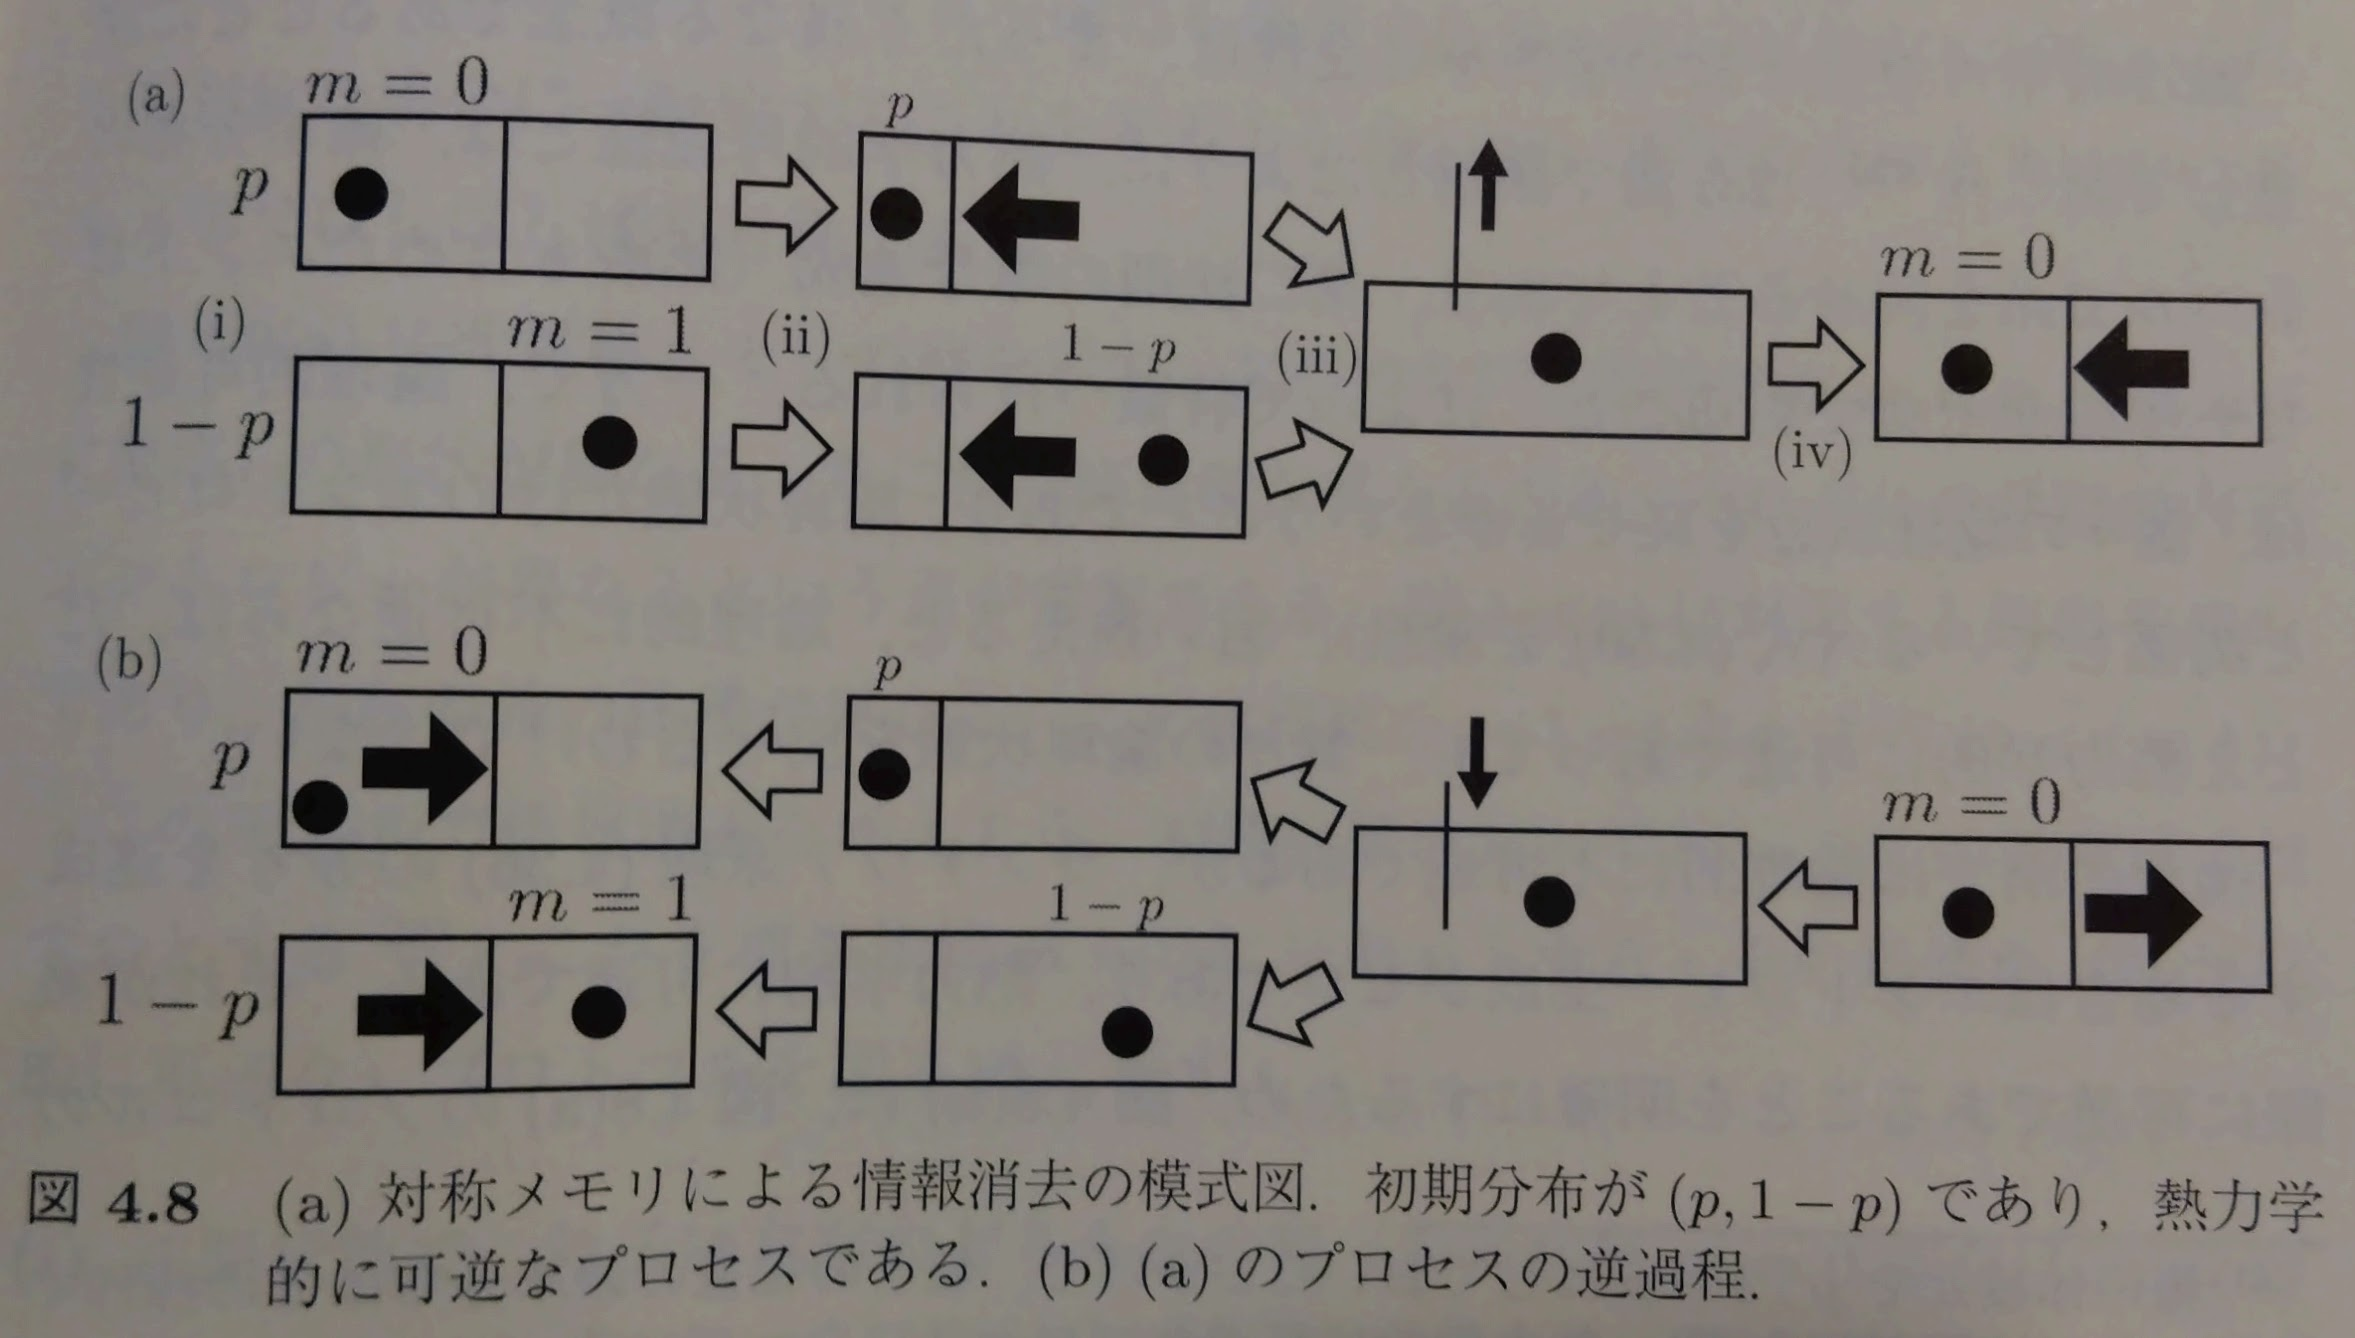
\includegraphics[width=0.4\columnwidth]{3-5-1.JPG}
    \caption{シラードエンジンの模式図。沙川先生の非平衡統計力学から引用。
    黒い点は理想気体粒子を表していて、これがある領域では圧力があると考える。}
\end{wrapfigure}

これはシラードエンジンというメモリを熱力学的に扱うモデルによって説明される。
\footnote{相当抽象化してるモデルになってるのでこれで一般的な場合をちゃんと扱えてるかどうかは私にはわからない。}
確率\(p\)で左に理想気体粒子が1つある 0 の状態にあり、
確率\(1-p\)で右に理想気体粒子が1つある 1 の状態にあるものとする。
初期状態では体積\(V\)の真ん中で区切られているものとする。

まず初めに左に粒子があるとき、準静的な圧縮で体積を\(pV\)にするのに必要な仕事は
\begin{equation*}
    W_2^{(0)} = \int_{V/2}^{pV} -pdV = -k_B T \int_{V/2}^{pV} \frac{dV}{V} = -k_B T \ln(2p)
\end{equation*}
その後仕切りを外して右側の壁を左に寄せていってまた半分にすると、
\begin{equation*}
    W_4 = \int_{V}^{V/2} -pdV = k_BT \ln 2
\end{equation*}
一方、初期状態として右に粒子があるときに(ii)の過程で必要な仕事は
\begin{equation*}
    W_2^{(1)} = \int_{V/2}^{(1-p)V}- pdV = -k_BT\ln(2(1-p))
\end{equation*}
なので消去に必要な仕事は
\begin{equation*}
    W = pW_2^{(0)} + (1-p)W_2^{(1)} + W_4 = k_B T \qty{-p\ln p - (1-p)\ln(1-p)} = k_B T H(p)
\end{equation*}
というように示せる。
エントロピーへの変換は準静的過程における熱力学第一法則
\begin{equation*}
    dU = -dW + TdS
\end{equation*}
を考えるとサイクルになっているので内部エネルギー変化\(dU\)はないことからできる。
これが下限になっているのは準静的過程での変化を使っているのに由来する。

進んだ補足をいくつか載せる。
体積を\(p:1-p\)にしないとこの操作により、
粒子の位置の確率分布は変化してしまい、
熱力学的に不可逆になってしまうかららしい。
また、このサイクルでは初めにどちらに粒子があるかがわかった状態で話をしている。
どちらに入っているかわからないときには観測をする必要がある。
すると観測にもエネルギーが必要となり、観測して情報を消去するときには
シャノンエントロピーではなく、相互情報量が下限になるそうである。

では実際の計算機ではどれくらいになっているかというと、
2000年の計算機で大体\(500k_B T\)程度である。

以下では情報の消去と計算の可逆性は同じものとして議論する。

この議論はいろいろと疑わしいが本文の流れに沿うため乗せる。
\begin{quotation}
    計算の不可逆性と情報の消去が等価であることと Landauer の原理を組み合わせると面白いことが言える。
    物理の理論は根本的に時間反転をすることができるためすべての過程は可逆である。
    もし、可逆過程のみで計算を行うことができるとすると、それは情報の消去をすることなしに計算をすることとなる。
    するとエネルギー消費の下限がなくなるため、エネルギー消費なしで計算することができるといえる。
\end{quotation}
まず計算の不可逆性と情報の消去は等価であるか疑わしい。
次に物理の理論は時間反転をすることができるというように言っているが、
時間反転対称性の破れた系は多くある。電子相関系でいうと交代磁性がその1つである。
当然熱力学が使える系はボルツマンのΗ定理といったように時間反転はできない。

\clearpage
\begin{wrapfigure}{r}[0pt]{0.4\columnwidth}
    \centering
    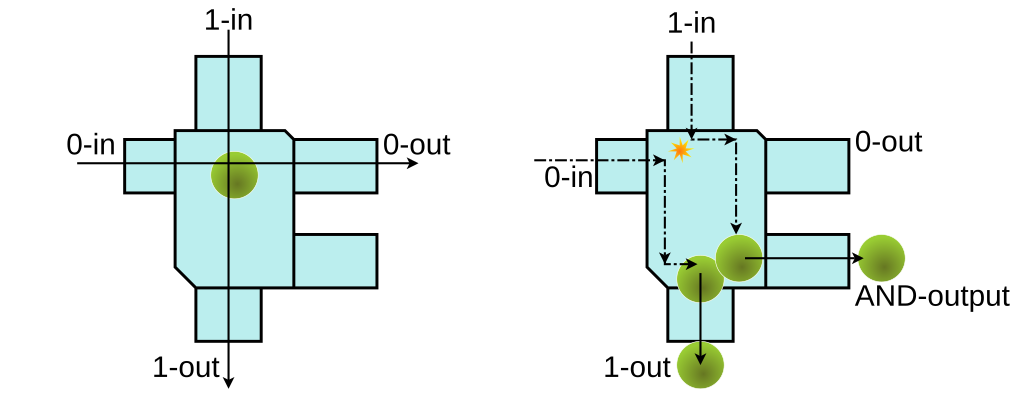
\includegraphics[width=0.4\columnwidth]{Toffoli_BilliardBall.png}
    \caption{ビリヤードコンピュータによる AND ゲート。余計な出力のための穴があって情報が失われないようになっている。}
    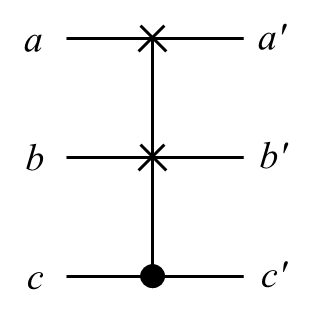
\includegraphics[width=0.3\columnwidth]{C-Swap.png}
    \caption{Fredkin (Controled-Swap) ゲート}
\end{wrapfigure}
いずれにせよ可逆計算というのは注目されていて、
どのようなモデルがあるかというのはいろいろと考えられてた。
その1つとして Fredkin のビリヤードコンピュータがある。
ビリヤードの玉の有無で情報ビットを表し、壁や玉同士の衝突によって計算を行うといったモデルである。
完璧にビリヤードの玉を突いて、様々な擾乱が無いという古典力学が完璧に成り立つという非現実的な仮定をしているものの、
セルオートマトンを用いたシミュレーションはできるのでそんなに悪くないモデルなのかもしれない。
ビリヤードコンピュータは回路モデルと等価となるように設計することができる。
その際に重要になるゲートが Fredkin (Controled-Swap)ゲートである。
このゲートは制御ビットが 1 のとき、上2のビットを入れ替えるというゲートである。
入れ替えの操作自体は2回連続で行うと元に戻るため、
Fredkin ゲートを連続させるともとの状態に戻ることから確かに可逆ゲートである(Excercise 3.29)。
教科書の図3.14は Fredkin ゲートになっている(Excercise 3.30)。

また、この Fredkin ゲートは AND, NOT, CROSSOVER そして FANOUT 関数をシミュレーションできる(fig. 3.16)。
この Fredkin ゲートを見ていったときにわかる特徴として、入力\(x\)に加え、
補助ビット\(a\)を用意して可逆ゲートに通すと望みの計算\(f(x)\)と副産物(garbage)である\(g(x)\)を出力することになるというのがわかる。

この副産物は適切に可逆ゲートを使うとこで計算時間をあまり変えずに取り除くことができる。
可逆ゲートとして計算結果に\(f(x)\)と副産物\(g(x)\)を出力するようなゲート\(G\)と CNOT ゲートを考える。
4つのレジスタ\((x,\,0,\,0,\,y)\)を舞台に計算をしていく。
古典計算においても CNOT ゲートは \((x,\,c) \rightarrow (x\oplus c,\,c)\)というように働く。
CNOT ゲートは\((0,\,c)\rightarrow (0 \oplus c,\, c)\)というように FANOUT ゲートとして使える。
なので次のような操作ができる。
\begin{equation*}
    (x,\,0,\,0,\,y)
    \overset{\text{FANOUT}}{\longrightarrow} (x,\,x,\,0,\,y)
    \overset{G}{\longrightarrow} (x,\,f(x),\,g(x),\,y)
    \overset{\text{CNOT}}{\longrightarrow} (x,\,x,\,g(x),\,y \oplus f(x))
    \overset{G^{-1}}{\longrightarrow} (x,\,0,\,0,\,y \oplus f(x))
\end{equation*}
\begin{enumerate}
    \item 第一レジスタを第二レジスタへとコピーする。
    \item 第二レジスタと第三レジスタを可逆ゲート\(G\)に通す。
    \item 第二レジスタを制御ビット、第四レジスタを目標ビットとして CNOT ゲートに通す。
    \item 第二レジスタと第三レジスタを可逆ゲート\(G^{-1}\)に通す。
\end{enumerate}
この過程を見ると途中で使った補助レジスタはそのままに目標の計算結果\(f(x)\)だけを取り出せているのがわかる。

つまり可逆でない計算であっても時間的・空間的リソースを出せば可逆にすることができるというのがわかる。
では負担すべきリソースの量はどのようになるか?
これは上の過程を見てわかるように非可逆ゲート1つにつき1つの Fredkin ゲートが必要となる。
また、補助ビットも元のビットの定数倍である。
そして補助ビットをもとに戻すのに定数倍の CNOT ゲートが必要となるため全体としては、
P や NP といった複雑性クラスは変更を受けない。
\\
\begin{tcolorbox}[title= 可逆半加算器]
    入力として\(x,\,y\)を受け取り、
    繰り上がりのビット\(c\)と\(x\oplus y\)を返すような
    \begin{equation*}
        (x,\,y,\,0,\,0) \rightarrow (x,\,y,\,c,\,x\oplus y)
    \end{equation*}
    となる可逆半加算器を作れ。
\end{tcolorbox}
このような操作をすればよい。
\begin{equation*}
    (x,\,y,\,0,\,0)
    \overset{\text{Toffoli}}{\longrightarrow} (x,\,y,\,0\oplus xy,\,0)
    \overset{\text{CNOT}}{\longrightarrow} (x,\,y,\,xy,\,0\oplus x)
    \overset{\text{CNOT}}{\longrightarrow} (x,\,x,\,xy,\,x\oplus y)
\end{equation*}
\begin{enumerate}
    \item 第一レジスタと第二レジスタを制御ビット、第三ビットを目標ビットにして Toffoli ゲートに通す。
    \item 第一レジスタを制御ビット、第四レジスタを目標ビットとして CNOT ゲートに通す。
    \item 第二レジスタを制御ビット、第四レジスタを目標ビットとして CNOT ゲートに通す。
\end{enumerate}
Toffoli ゲートが可逆であるのは fig.3.17 よりわかる。

ここで出てきた可逆ゲートである Toffoli ゲートについてみていく。
このゲートはユニバーサル計算ができる。
というのも
\begin{equation*}
    (x,\,y,\,1)
    \overset{\text{Toffoli}}{\longrightarrow} (x,\,y,\,\neg (xy))
\end{equation*}
となり、 NAND ゲートとなるからである(fig. 3.18)。
この Toffoli ゲートに関する計算モデルは Chapter 7 で行っていく。
理想的なビリヤードコンピュータモデルではエネルギーなしで計算できるのがわかるが、
そこでも Toffoli ゲートはエネルギー消費なしで計算できることを示す。
\begin{tcolorbox}[title = Fredkin と Toffoli の等価性]
    Toffoli ゲートをシミュレーションするには少なくともいくつの Fredkin ゲートを使えばよいか?
    Fredkin ゲートをシミュレーションするには少なくともいくつの Toffoli ゲートを使えばよいか?
\end{tcolorbox}
Toffoli ゲートから Fredkin ゲートを再現するにはこのようにすればよい。
\begin{equation*}\begin{split}
        &(c,\,x,\,y)\\
        &\overset{\text{contorl:1,2 target:3}}{\longrightarrow} (c,\,x,\,y\oplus cx)\\
        &\overset{\text{contorl:1,3 target:2}}{\longrightarrow} (c,\,x \oplus c(y\oplus cx),\,y \oplus cx)
        =(c,\,\bar{c}x\oplus cy,\,y\oplus cx)\\
        &\overset{\text{contorl:1,2 target:3}}{\longrightarrow} (c,\,\bar{c}x\oplus cy,\, cy \oplus y\oplus cx)
        =(c,\,\bar{c}x \oplus cy,\,\bar{c}y\oplus cx)
\end{split}\end{equation*}
\begin{enumerate}
    \item 第三レジスタと第四レジスタを制御ビット、第二ビットを目標ビットにして Toffoli ゲートに通す。
    \item 第一レジスタと第二レジスタを制御ビット、第三ビットを目標ビットにして Toffoli ゲートに通す。
    \item 第三レジスタと第四レジスタを制御ビット、第二ビットを目標ビットにして Toffoli ゲートに通す。
\end{enumerate}
見ずらいかもしれないが、これにより Fredkin ゲートとなる。なので多く見積もっても3つは必要である。

逆はこのようにすればよいらしい。
% \begin{equation*}\begin{split}
%     &(x,\,y,\,c,\,0)\\
%     &\overset{\text{contorl:1 target:3,4}}{\longrightarrow} (x,\,y,\,c\bar{x} + 0x,\,\bar{x}0 + cx)
%     =(x,\,y,\,c\bar{x},\,cx)\\
%     &\overset{\text{contorl:2 target:3,4}}{\longrightarrow}(x,\,y,\,c\bar{x}\bar{y} + cxy,\,cxy + cx\bar{y})
%     =\qty(x,\,y,\,c(xy + \bar{x}\bar{y}),\, c(x\bar{y} + \bar{x}y))\\
%     &\overset{\text{contorl:1 target:3,4}}{\longrightarrow}\qty(x,\,y,\,c(xy +\bar{x}\bar{y})\bar{x} + c(x\bar{y}+\bar{x}y)x,\,c(x\bar{y}+\bar{x}y)x+c(xy+\bar{x}\bar{y})\bar{x})
% \end{split}\end{equation*}
\begin{enumerate}
\item 第三レジスタと第四レジスタを制御ビット、第二ビットを目標ビットにして Toffoli ゲートに通す。
\item 第一レジスタと第二レジスタを制御ビット、第三ビットを目標ビットにして Toffoli ゲートに通す。
\item 第三レジスタと第四レジスタを制御ビット、第二ビットを目標ビットにして Toffoli ゲートに通す。
\end{enumerate}
% これの第4レジスタについて、
% \begin{equation*}
%     c(x\bar{y} + \bar{x}y)\bar{x} +  c(xy + \bar{x}\bar{y})x
%     = c (x\bar{y} + x\bar{y})
% \end{equation*}

ここでエネルギー消費なしで計算するという概念には重大な注意が必要である。
これ見てきたようにこのような計算はノイズにとても敏感であるため、
このノイズを取り除くのになんらかの形で誤り訂正をする必要がある。
そのような誤り訂正をする際には、思い通りの計算をしているか確かめるため、
系の状態を測定する必要がある。ここでエネルギーを消費してしまう。
\footnote{なので本質的に可逆計算はここでエネルギーを消費してしまうようである。}
また実際のリソースが有限の計算機では、
誤り訂正に使う情報というのはいつまでも保っておくことはできないため、
この情報を消去する必要がある。ここで Landauer の原理よりエネルギーを消費する必要が生じる。

可逆計算についての話から何を結論づけられるだろうか?
\begin{enumerate}
    \item 情報の消去にはエネルギーを消費する。
    \item 可逆的に計算ができるといった時にはエネルギーを消費することはない。
    \item 非可逆回路であっても可逆回路に直すことができて、計算複雑性も変わらないことが多い。
\end{enumerate}
といったことである。

この結果は物理学者やハードウェアエンジニアにとっては、
可逆計算により熱散逸をなくせるという事実はいいニュースである。
そして、ここの話は Maxwell' demon という問題への解決へとつながっていく。
計算機科学者にとっては、
自然界は本来可逆であるのだから
非可逆な計算モデルであるチューリングマシンよりもっとよい複雑性クラスについて議論することができるのではないかというのがある。

\section{Perspective on computer science}
この章を締めるのに計算機科学全体の地図において、
量子コンピューターはどのような立ち位置にあるのかをざっと見ていく。

この章ではチューリングマシンを計算のモデルとして議論していった。
大規模並列計算機、DNA 計算機、アナログコンピュータのようなチューリングマシンではないようなモデルにおける計算力というのはどのようなものだろうか。
そしてこれらは量子計算機と間接的に比較してどうだろうか?
いま存在している大抵の計算機といったときには、中央にある処理ユニットに一個一個の命令を順に実行させるようなシリアル計算機である。
これと対称的に、並列計算機は同時に命令を同時に処理していくようなものであり、応用例によっては時間とお金を節約するような可能性を秘めている。
そうはいっても、並列計算機はチューリングマシンにたいして有利な点というのは実はない。
というのもチューリングマシンは並列計算を多項式時間、同じ物理的なリソースでできるからである。
この物理的なリソースは時間リソースと空間リソースの2つになっていて、これらはトレードオフになっている。
なので有利な点はないというわけだ。

大規模並列計算の面白い例として、DNA 計算機というのがある。
DNA は A, C, G, T の4つのヌクレオチドからなっていて、
AC, CG のペアを作って2重螺旋を作る。
この二重螺旋が入った溶液に開始コドンと終止コドンを増やしたり、
ポリメラーゼ連鎖反応により特定の配列を増やしたりする。
その後、重さが違うことを利用して DNA 鎖を分離して、
pH や温度を変えることにより2重螺旋を1重螺旋にする。
制限酵素により DNA を切断し、そうしてできた試料が望みの配列になっているかをチェックする。
こういったようにして DNA の配列をいじくって計算をするというものである。

ハミルトン有向路問題は3.2.2で見たハミルトン閉路問題の変形であり、NP 完全である。
\begin{tcolorbox}[title = ハミルトン有向路問題]
    \(N\)個の頂点を持つ有効グラフ\(G\)において、
    各頂点に厳密に1度だけ入り、辺の向きに沿って2角特定の頂点\(j_1\)と\(j_N\)の間に経路があるかを
    判定する問題。
\end{tcolorbox}

\end{document}